\section{Lec 19}
We see that with this metric, the light cones do not close up.\par
\bigskip
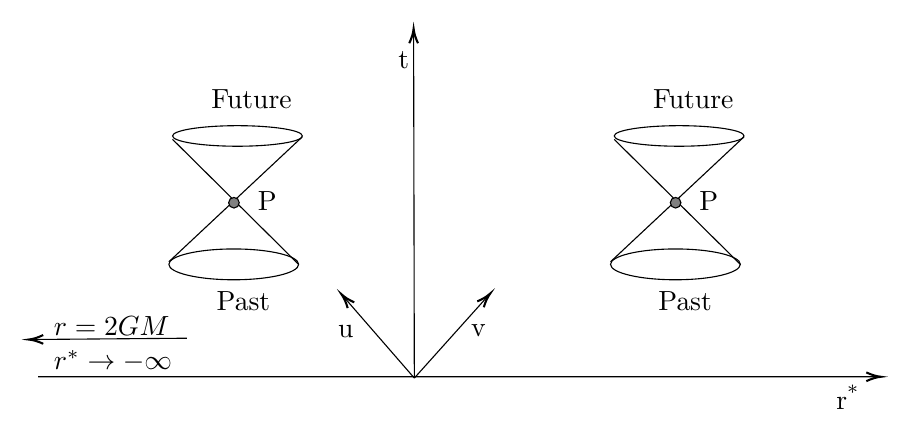
\begin{tikzpicture}[x=0.48pt,y=0.48pt,yscale=-1,xscale=1]
\draw    (304.3,272) -- (303.75,11) ;
\draw [shift={(303.75,9)}, rotate = 89.88] [color={rgb, 255:red, 0; green, 0; blue, 0 }  ][line width=0.75]    (10.93,-3.29) .. controls (6.95,-1.4) and (3.31,-0.3) .. (0,0) .. controls (3.31,0.3) and (6.95,1.4) .. (10.93,3.29)   ;
\draw    (21,271) -- (653.5,271.03) ;
\draw [shift={(655.5,271.03)}, rotate = 180] [color={rgb, 255:red, 0; green, 0; blue, 0 }  ][line width=0.75]    (10.93,-3.29) .. controls (6.95,-1.4) and (3.31,-0.3) .. (0,0) .. controls (3.31,0.3) and (6.95,1.4) .. (10.93,3.29)   ;
\draw    (454.79,92.31) -- (549.71,186.4) ;
\draw    (552.5,90.38) -- (452,184.47) ;
\draw   (452,186.4) .. controls (452,179.99) and (473.87,174.8) .. (500.85,174.8) .. controls (527.84,174.8) and (549.71,179.99) .. (549.71,186.4) .. controls (549.71,192.81) and (527.84,198) .. (500.85,198) .. controls (473.87,198) and (452,192.81) .. (452,186.4) -- cycle ;
\draw   (454.79,89.73) .. controls (454.79,85.46) and (476.66,82) .. (503.65,82) .. controls (530.63,82) and (552.5,85.46) .. (552.5,89.73) .. controls (552.5,94) and (530.63,97.47) .. (503.65,97.47) .. controls (476.66,97.47) and (454.79,94) .. (454.79,89.73) -- cycle ;
\draw  [fill={rgb, 255:red, 128; green, 128; blue, 128 }  ,fill opacity=1 ] (497,140) .. controls (497,137.79) and (498.79,136) .. (501,136) .. controls (503.21,136) and (505,137.79) .. (505,140) .. controls (505,142.21) and (503.21,144) .. (501,144) .. controls (498.79,144) and (497,142.21) .. (497,140) -- cycle ;
\draw    (122.29,92.31) -- (217.21,186.4) ;
\draw    (220,90.38) -- (119.5,184.47) ;
\draw   (119.5,186.4) .. controls (119.5,179.99) and (141.37,174.8) .. (168.35,174.8) .. controls (195.34,174.8) and (217.21,179.99) .. (217.21,186.4) .. controls (217.21,192.81) and (195.34,198) .. (168.35,198) .. controls (141.37,198) and (119.5,192.81) .. (119.5,186.4) -- cycle ;
\draw   (122.29,89.73) .. controls (122.29,85.46) and (144.16,82) .. (171.15,82) .. controls (198.13,82) and (220,85.46) .. (220,89.73) .. controls (220,94) and (198.13,97.47) .. (171.15,97.47) .. controls (144.16,97.47) and (122.29,94) .. (122.29,89.73) -- cycle ;
\draw  [fill={rgb, 255:red, 128; green, 128; blue, 128 }  ,fill opacity=1 ] (164.5,140) .. controls (164.5,137.79) and (166.29,136) .. (168.5,136) .. controls (170.71,136) and (172.5,137.79) .. (172.5,140) .. controls (172.5,142.21) and (170.71,144) .. (168.5,144) .. controls (166.29,144) and (164.5,142.21) .. (164.5,140) -- cycle ;
\draw    (133,242) -- (16,242.98) ;
\draw [shift={(14,243)}, rotate = 359.52] [color={rgb, 255:red, 0; green, 0; blue, 0 }  ][line width=0.75]    (10.93,-3.29) .. controls (6.95,-1.4) and (3.31,-0.3) .. (0,0) .. controls (3.31,0.3) and (6.95,1.4) .. (10.93,3.29);
%Straight Lines [id:da29574799350771797] 
\draw    (304.3,272) -- (360.11,209.81) ;
\draw [shift={(361.45,208.32)}, rotate = 131.9] [color={rgb, 255:red, 0; green, 0; blue, 0 }  ][line width=0.75]    (10.93,-3.29) .. controls (6.95,-1.4) and (3.31,-0.3) .. (0,0) .. controls (3.31,0.3) and (6.95,1.4) .. (10.93,3.29)   ;
%Straight Lines [id:da5479056018248073] 
\draw    (304.3,272) -- (250.75,210.4) ;
\draw [shift={(249.43,208.89)}, rotate = 49] [color={rgb, 255:red, 0; green, 0; blue, 0 }  ][line width=0.75]    (10.93,-3.29) .. controls (6.95,-1.4) and (3.31,-0.3) .. (0,0) .. controls (3.31,0.3) and (6.95,1.4) .. (10.93,3.29)   ;


\draw (290.38,24) node [anchor=north west][inner sep=0.75pt]   [align=left] {t};
\draw (620,275) node [anchor=north west][inner sep=0.75pt]   [align=left] {r\textsuperscript{*}};
% Text Node
\draw (517,130) node [anchor=north west][inner sep=0.75pt]   [align=left] {P};
% Text Node
\draw (482,53) node [anchor=north west][inner sep=0.75pt]   [align=left] {Future};
% Text Node
\draw (486,205) node [anchor=north west][inner sep=0.75pt]   [align=left] {Past};
% Text Node
\draw (184.5,130) node [anchor=north west][inner sep=0.75pt]   [align=left] {P};
% Text Node
\draw (149.5,53) node [anchor=north west][inner sep=0.75pt]   [align=left] {Future};
% Text Node
\draw (153.5,205) node [anchor=north west][inner sep=0.75pt]   [align=left] {Past};
% Text Node
\draw (31,224) node [anchor=north west][inner sep=0.75pt]   [align=left] {$r = 2GM$\\$r^{*} \to  - \infty$};
% Text Node
\draw (245,230.22) node [anchor=north west][inner sep=0.75pt]   [align=left] {u};
% Text Node
\draw (345,229.89) node [anchor=north west][inner sep=0.75pt]   [align=left] {v};
\end{tikzpicture}
\bigskip
The big \emph{con } is that the surface of the \emph{r\textsubscript{S}} is positioned to infinity.\par
Next move is to define coordinates adapted to light-like geodesics
\begin{align}
	v & \equiv t+ r^{*}\\
	u & \equiv t - r^{*} 
\end{align}
then \emph{infalling} radial light-like geodesics are characterized by $v =$ constant, the \emph{outgoing} ones $u=$ constant


\subsection{Eddington-Finkelstein}
Now we want to have a coordinates change from $\left( t,r \right) \to \left( v,r \right)$, these are EF coordinates. \emph{v} is good to discuss infalling geodesics.
\[
dv = dt + dr^{*} = dt + \frac{dr}{1- \frac{2GM}{r}}
\]
\begin{align}
	ds^{2} &= - \left( 1 - \frac{2GM}{r} \right)dt^{2} + \left( 1- \frac{2GM}{r} \right)^{-1}dr^{2} = \\
	       & = - \left( 1- \frac{2GM}{r} \right) \left( dv - \frac{dr}{1 - \frac{2GM}{r}} \right)^{2} + \left( 1 - \frac{2GM}{r} \right)^{-1} dr^{2} = \\
	       & = - \left( 1 - \frac{2GM}{r} \right)dv^{2} + \left( dvdr-drdv \right) + r^{2}d\Omega .
\end{align}
In EF coordinates the condition for radial null curves is solved by
\begin{equation}
\frac{d v}{d r} = \begin{cases}
0,   \text{ (infalling) }\\
2 \left( 1 - \frac{2GM}{r} \right)^{-1} , \text{ outgoing }\\
\end{cases}
\end{equation}
In this coordinates system the light cones remain well behaved at $r=r_{S}$. But we see that light-cones tilts, such that for $r<2GM$ all-future directed paths are in the directions of decreasing \emph{r}.\par
\bigskip

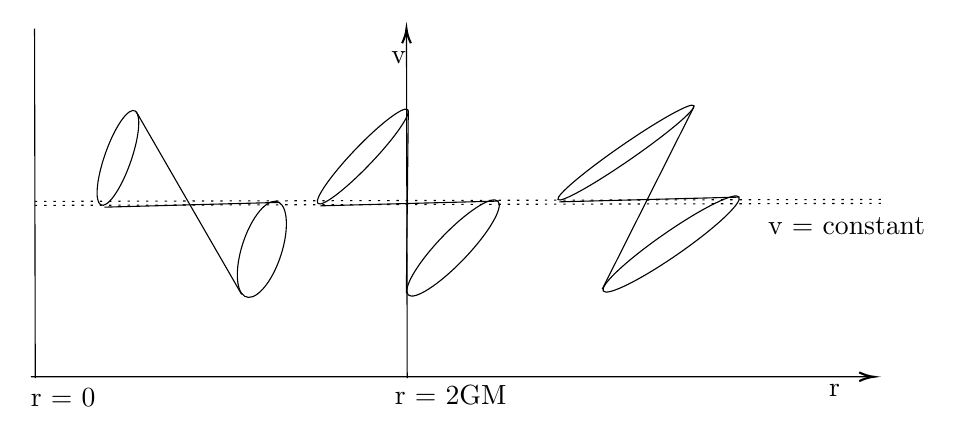
\begin{tikzpicture}[x=0.48pt,y=0.48pt,yscale=-1,xscale=1]
%Straight Lines [id:da6124197854166261]
\draw    (304.3,272) -- (303.75,11) ;
\draw [shift={(303.75,9)}, rotate = 89.88] [color={rgb, 255:red, 0; green, 0; blue, 0 }  ][line width=0.75]    (10.93,-3.29) .. controls (6.95,-1.4) and (3.31,-0.3) .. (0,0) .. controls (3.31,0.3) and (6.95,1.4) .. (10.93,3.29)   ;
%Straight Lines [id:da9536673650889413]
\draw    (21,271) -- (653.5,271.03) ;
\draw [shift={(655.5,271.03)}, rotate = 180] [color={rgb, 255:red, 0; green, 0; blue, 0 }  ][line width=0.75]    (10.93,-3.29) .. controls (6.95,-1.4) and (3.31,-0.3) .. (0,0) .. controls (3.31,0.3) and (6.95,1.4) .. (10.93,3.29)   ;
%Straight Lines [id:da08490630321795567]
\draw    (238.98,142.34) -- (372.58,138.77) ;
%Straight Lines [id:da879557342815412]
\draw    (305.12,70.39) -- (303.66,208.05) ;
\draw   (305.05,209.39) .. controls (300.42,204.96) and (311.79,185.56) .. (330.44,166.06) .. controls (349.08,146.56) and (367.95,134.34) .. (372.58,138.77) .. controls (377.21,143.2) and (365.85,162.59) .. (347.2,182.09) .. controls (328.56,201.59) and (309.69,213.81) .. (305.05,209.39) -- cycle ;
\draw   (237.12,140.56) .. controls (234.03,137.61) and (246.65,119.41) .. (265.3,99.91) .. controls (283.94,80.41) and (301.56,66.99) .. (304.65,69.94) .. controls (307.74,72.89) and (295.12,91.09) .. (276.47,110.59) .. controls (257.83,130.1) and (240.21,143.51) .. (237.12,140.56) -- cycle ;
\draw    (24.3,272) -- (23.75,9) ;
\draw  [dash pattern={on 0.84pt off 2.51pt}]  (24.02,139) -- (661,137.5)(24.03,142) -- (661,140.5) ;
\draw    (418.79,139.34) -- (554.15,135.77) ;
\draw    (520.35,67.39) -- (451.11,205.05) ;
\draw   (451.85,206.39) .. controls (449.4,201.96) and (470.31,182.56) .. (498.56,163.06) .. controls (526.81,143.56) and (551.69,131.34) .. (554.15,135.77) .. controls (556.6,140.2) and (535.68,159.6) .. (507.44,179.1) .. controls (479.19,198.6) and (454.3,210.82) .. (451.85,206.39) -- cycle ;
\draw   (417.81,137.56) .. controls (416.17,134.61) and (437.75,116.4) .. (466,96.9) .. controls (494.24,77.4) and (518.47,63.98) .. (520.1,66.94) .. controls (521.74,69.89) and (500.16,88.1) .. (471.91,107.6) .. controls (443.67,127.1) and (419.44,140.52) .. (417.81,137.56) -- cycle ;
\draw    (76.41,143.34) -- (207.91,139.77) ;
\draw    (100.27,71.39) -- (179.68,209.05) ;
\draw   (181.86,210.38) .. controls (174.63,205.96) and (174.6,186.56) .. (181.8,167.06) .. controls (188.99,147.56) and (200.68,135.34) .. (207.91,139.77) .. controls (215.14,144.2) and (215.17,163.59) .. (207.98,183.09) .. controls (200.79,202.59) and (189.09,214.81) .. (181.86,210.38) -- cycle ;
\draw   (73.5,141.56) .. controls (68.68,138.61) and (70.6,120.41) .. (77.8,100.91) .. controls (84.99,81.41) and (94.73,67.99) .. (99.55,70.94) .. controls (104.37,73.89) and (102.44,92.09) .. (95.25,111.59) .. controls (88.06,131.09) and (78.32,144.51) .. (73.5,141.56) -- cycle ;
\draw (290.38,24) node [anchor=north west][inner sep=0.75pt]   [align=left] {v};
\draw (620,275) node [anchor=north west][inner sep=0.75pt]   [align=left] {r};
\draw (293,276) node [anchor=north west][inner sep=0.75pt]   [align=left] {r = 2GM};
\draw (19,278) node [anchor=north west][inner sep=0.75pt]   [align=left] {r = 0};
\draw (574,149) node [anchor=north west][inner sep=0.75pt]   [align=left] {v = constant};
\end{tikzpicture}
\bigskip

The surface at $r=r_{S}$, acts as a point of no return, once a test particle passes it, it can never come back, An event horizon  is a surface past which particles can never escape to infinity. Since nothing can escape it, we cannot see inside, so it's a \emph{black hole}, which is a region of spacetime separated from infinity by event horizon.\par

In $\left( v,r \right)$ coordinates system we can cross the event horizon on future-directed paths, but not on past-directed ones. Well, wtf,\par
If we have chosen \emph{u} instead of \emph{v} the metric would have been
\begin{gather*}
	\left( t,r \right) \to \left( u,r \right) \\
	du = dt- dr^{*} = dt - \frac{dr}{1 - \frac{2GM}{r}} \\
	\begin{cases}
		\frac{d v}{d r} =-2 \left(  1 - \frac{2GM}{r} \right)^{-1} & \text{  infalling }\\
		du = 0 &\text{  outgoing }
	\end{cases}
\end{gather*}
and the metric becomes
\begin{equation}
ds^{2} = - \left( 1 - \frac{2GM}{r} \right)du^{2} - \left(  dudr + drdu \right) + r^{2}d\Omega 
\end{equation}

Now we can pass through the event horizon but this time along past-directed curves.\par
\bigskip
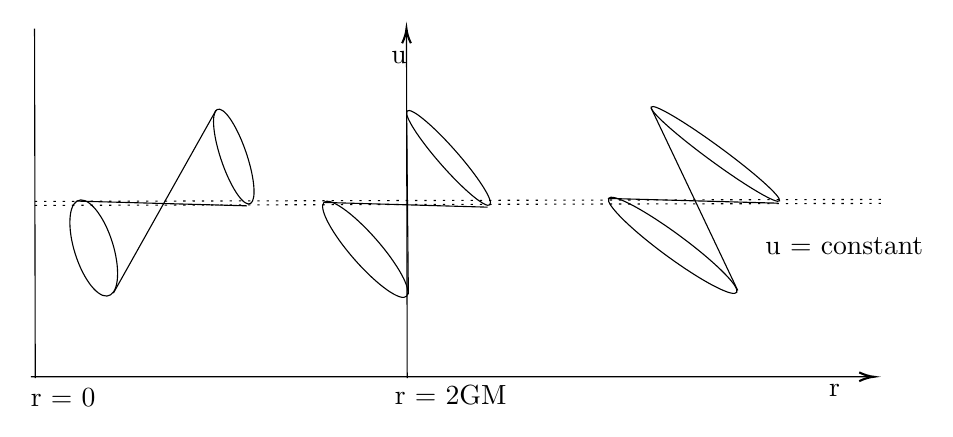
\begin{tikzpicture}[x=0.48pt,y=0.48pt,yscale=-1,xscale=1]
\draw    (304.3,272) -- (303.75,11) ;
\draw [shift={(303.75,9)}, rotate = 89.88] [color={rgb, 255:red, 0; green, 0; blue, 0 }  ][line width=0.75]    (10.93,-3.29) .. controls (6.95,-1.4) and (3.31,-0.3) .. (0,0) .. controls (3.31,0.3) and (6.95,1.4) .. (10.93,3.29)   ;
\draw    (21,271) -- (653.5,271.03) ;
\draw [shift={(655.5,271.03)}, rotate = 180] [color={rgb, 255:red, 0; green, 0; blue, 0 }  ][line width=0.75]    (10.93,-3.29) .. controls (6.95,-1.4) and (3.31,-0.3) .. (0,0) .. controls (3.31,0.3) and (6.95,1.4) .. (10.93,3.29)   ;
\draw    (364.85,143.34) -- (241.57,139.77) ;
\draw    (303.83,71.39) -- (305.17,209.05) ;
\draw   (303.89,210.38) .. controls (308.16,205.95) and (297.68,186.56) .. (280.47,167.06) .. controls (263.26,147.56) and (245.84,135.34) .. (241.57,139.77) .. controls (237.29,144.2) and (247.78,163.6) .. (264.99,183.1) .. controls (282.2,202.6) and (299.61,214.81) .. (303.89,210.38) -- cycle ;
\draw   (366.57,141.56) .. controls (369.42,138.6) and (357.78,120.4) .. (340.57,100.9) .. controls (323.37,81.4) and (307.11,67.99) .. (304.26,70.94) .. controls (301.41,73.9) and (313.05,92.1) .. (330.25,111.6) .. controls (347.46,131.1) and (363.72,144.51) .. (366.57,141.56) -- cycle ;
\draw    (24.3,272) -- (23.75,9) ;
\draw  [dash pattern={on 0.84pt off 2.51pt}]  (24.02,139) -- (661,137.5)(24.03,142) -- (661,140.5) ;
\draw    (583.66,140.34) -- (455.85,136.77) ;
\draw    (487.76,68.39) -- (553.14,206.05) ;
\draw   (552.44,207.39) .. controls (554.76,202.95) and (535.01,183.55) .. (508.34,164.05) .. controls (481.66,144.55) and (458.16,132.34) .. (455.85,136.77) .. controls (453.54,141.2) and (473.28,160.6) .. (499.95,180.1) .. controls (526.63,199.6) and (550.13,211.82) .. (552.44,207.39) -- cycle ;
\draw   (584.59,138.56) .. controls (586.13,135.6) and (565.76,117.4) .. (539.08,97.9) .. controls (512.41,78.4) and (489.54,64.99) .. (487.99,67.94) .. controls (486.45,70.9) and (506.82,89.1) .. (533.49,108.6) .. controls (560.17,128.1) and (583.04,141.51) .. (584.59,138.56) -- cycle ;
\draw    (183.58,142.34) -- (55.65,138.77) ;
\draw    (160.37,70.39) -- (83.11,208.05) ;
\draw   (80.99,209.38) .. controls (88.02,204.96) and (88.05,185.56) .. (81.06,166.06) .. controls (74.06,146.56) and (62.68,134.34) .. (55.65,138.77) .. controls (48.62,143.2) and (48.59,162.59) .. (55.59,182.09) .. controls (62.59,201.59) and (73.96,213.81) .. (80.99,209.38) -- cycle ;
\draw   (186.42,140.56) .. controls (191.1,137.61) and (189.23,119.41) .. (182.23,99.91) .. controls (175.24,80.41) and (165.76,66.99) .. (161.08,69.94) .. controls (156.39,72.89) and (158.26,91.09) .. (165.26,110.59) .. controls (172.26,130.09) and (181.73,143.51) .. (186.42,140.56) -- cycle ;
\draw (290.38,24) node [anchor=north west][inner sep=0.75pt]   [align=left] {u};
\draw (620,275) node [anchor=north west][inner sep=0.75pt]   [align=left] {r};
\draw (293,276) node [anchor=north west][inner sep=0.75pt]   [align=left] {r = 2GM};
\draw (19,278) node [anchor=north west][inner sep=0.75pt]   [align=left] {r = 0};
\draw (572,164) node [anchor=north west][inner sep=0.75pt]   [align=left] {u = constant};
\end{tikzpicture}
\bigskip

So, we can follow either future or past directed geodesics through $r_{S}$, but we arrive at different places. If we keep \emph{v} constant and decrease \emph{r} we must have $t \to + \infty$, while for \emph{u} constant we get $t \to  -\infty$.

\paragraph{Something to digest BHs} First, external geometry of a black hole is the Schwarzschild solution valid for any star or planet, this means BHs are not cosmic vacuum cleaners. \par
Second, if I did understand, it is technically possible escape a Newtonian BH, indeed \emph{c} in here is just a number, and while light can't escape the BH travelling inertially, it could be accelerated by something and manage to escape. While in GR, inside the event horizon, the geometry of the spacetime is curved in such a way that all paths lead inward. \par

\subsection{Kruskal-Szekeres coordinates}
Enough with light-like geodesics, now we try with space-like geodesics. A first guess one could do is to use both \emph{u,v}. 
\begin{gather*}
v = t + r^{*} \\
u = t - r^{*}\\
dv = dt + dr^{*} = dt + \frac{d r}{ 1 - \frac{2GM}{r}}\\
du = dt - dr^{*} = \ldots 
\end{gather*}
we see 
\begin{gather*}
dt = \frac{du + dv}{2} \\
dr = \left( \frac{du-dv}{2} \right)\left( 1- \frac{2GM}{r} \right)
\end{gather*}
so the metric becomes
\begin{align}
	ds^{2} &= - \left( 1- \frac{2GM}{r} \right)dt^{2} + \left( 1 - \frac{2GM}{r} \right)^{-1} dr^{2} = \\
	       &= - \left( 1 - \frac{2GM}{r}  \right)\left( \frac{du + dv}{2} \right)^{2} + \left( 1 - \frac{2GM}{r} \right) ^{+1} \left( \frac{du - dv}{2} \right)^{2} = \\
	       &= - \left( 1 - \frac{2GM}{r} \right)dudv
\end{align}
so for $r \to  2GM$, $r^{*}\to  -\infty$, $v \to  -\infty$ and $u \to +\infty$.\par
We can make an improvement, since in this coordinates \emph{r\textsubscript{S}} is at infinity like at the start. We choose new coordinates that are
\begin{gather*}
u^{\prime } = -e ^{- \frac{u}{4GM}} \\
v^{\prime } = + e ^{\frac{v}{4GM}}\\
du^{\prime } = \frac{1}{4GM} e^{-\frac{u}{4GM}}du\\
dv^{\prime } = \frac{1}{4GM} e^{+\frac{v}{4GM}}dv
\end{gather*}
this makes
\begin{align}
	dudv &= 16G^{2}M^{2} e^{ \frac{u-v}{4GM}} du^{\prime }dv^{\prime }\\
	     &\left( \frac{u-v}{4GM} = -\frac{r^{*}}{2GM} \right)\footnotemark \\
	     &=16G^{2}M^{2} e^{ -\frac{1}{2GM} \left( r + 2GM \text{ln}\left( \frac{r}{2GM} -1 \right)	 \right)} du^{\prime }dv^{\prime }
\end{align}
\footnotetext{using this particular substitution makes things easier.}
the metric becomes
\begin{equation}
ds^{2} = \frac{-32G^{3}M^{3}}{r} e ^{ -\frac{r}{2GM}} du^{\prime }dv^{\prime }
\end{equation}
this does not explode at $r = r_{S}$.\par
Reminder: we used the notation $2dudv$ that should be instead $dudv +dvdu$, because tensor product does not commute.\par
Coordinates $u^{\prime }$ and $v^{\prime }$ are null coordinates, since their partial derivatives are null vectors. We have four partial derivatives vectors (two null and two space-like) as basis for the tangent space. We prefer work with a system where coordinates are one time-like and the others three space-like. We define
\begin{gather*}
T = \frac{1}{2} \left( v^{\prime }+u^{\prime } \right) \\
R = \frac{1}{2} \left( v^{\prime }-u^{\prime } \right)
\end{gather*}
these give us
\begin{equation}
ds^{2 } = \frac{32G^{3}M^{3}}{r}e^{-\frac{r}{2GM}}\left( -dT^{2}+dR^{2} \right)
\end{equation}
where \emph{r} is defined from
\begin{equation}
T^{2}-R^{2} = \left( 1- \frac{r}{2GM} \right)e^{\frac{r}{2GM}}
\end{equation}
These coordinates are the Kruskal-Szekeres coordinates, $\left( T,R,\theta,\phi  \right)$.\par
Radial null curves, here, or light-like geodesics are
\begin{equation}
T = \pm R + \text{ const }
\end{equation}
while event horizon is at
\begin{equation}\label{eq:t=r}
T = \pm R
\end{equation}
consistent with being a null surface.\par
Surfaces are $r =$ constant so
\begin{equation}
T^{2} - R^{2} = \text{ constant }
\end{equation}
these looks like hyperbolae in \emph{R-T} plane.\par
Surfaces of constant \emph{t} are given by
\begin{equation}
\frac{T}{R} = \text{ tanh }\left( \frac{t}{4GM} \right)
\end{equation}
this defines straight lines through the origin with slope given by hyper-tangent. For $t\to \infty$ it becomes eq,\ref{eq:t=r}.\par
In this diagram each point on the diagram is a two-sphere, it represent the maximal extension of the Schwarzschild geometry.
We see that $-\infty < R < +\infty$ and $T^{2}< R^{2 }+1$.
\begin{figure}[h]
\centering
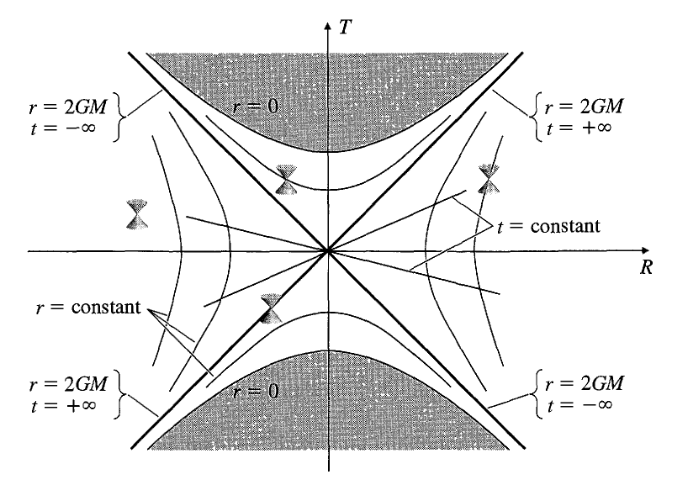
\includegraphics[width=\linewidth]{imm/ksdiagram.png}
\caption{Kruskal diagram}
\label{imm:ksdiagram}
\end{figure}
It is convenient to divide the diagram in 4 regions:
\begin{itemize}
\item Region I corresponds to $r>2GM$
\item With future directed light-like geodesics we reach region II
\item With past ones we reach region III
\item With space-like geodesics one gets to region IV
\end{itemize}
Definitions that relate (T,R) to (t,r) are good only in region I.\par
Region II is a \emph{black hole}, every future-directed path there hits $r=0$.\par
Region III is the time reversed of region II, could be the \emph{ white hole}. A singularity in the past from which everything appears to spring.\par
Region IV, cannot be reached from our region and viceversa. It is a mirror image of region I and could be reached by a wormhole.
\begin{figure}[h]
\centering
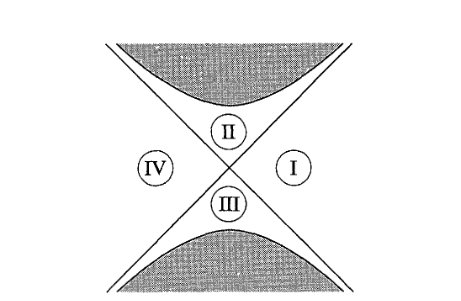
\includegraphics[width=\linewidth]{imm/kregion.png}
\caption{Regions of the kruskal diagram}
\label{imm:kregion.png}
\end{figure}





























